\documentclass[conference]{IEEEtran}
\IEEEoverridecommandlockouts
% The preceding line is only needed to identify funding in the first footnote. If that is unneeded, please comment it out.
\usepackage{cite}
\usepackage{amsmath,amssymb,amsfonts}
\usepackage{algorithmic}
\usepackage{graphicx}
\usepackage{textcomp}
\usepackage{xcolor}
\usepackage{subcaption}
\usepackage[hyphens]{url} 
\def\BibTeX{{\rm B\kern-.05em{\sc i\kern-.025em b}\kern-.08em
    T\kern-.1667em\lower.7ex\hbox{E}\kern-.125emX}}
\begin{document}

\title{Análise Preditiva Aplicada à Identificação de Fraudes em Seguros Automotivos
}

\author{\IEEEauthorblockN{Gabriel Estevão N. Sobrinho, Letícia T. Lott, Luana G. Fleury,\\ Rafael F. Barra, Yan R. Nalon}
\IEEEauthorblockA{\textit{Instituto de Ciências Exatas e Informática (ICEI)} \\
\textit{PUC Minas}\\
Belo Horizonte, Brasil \\
\{gensobrinho, lott.ltc, luana.fleury4, rafafbarra, yanrnalon\}@gmail.com}
}

\maketitle

\begin{abstract}
A detecção de fraudes em pedidos de seguros automotivos é fundamental para mitigar prejuízos financeiros e manter a eficiência operacional de seguradoras. Este estudo avalia o desempenho de quatro modelos de aprendizado de máquina (Regressão Logística, Naïve Bayes, Máquina de Vetores de Suporte (SVM) e Floresta de Decisão) na identificação de pedidos fraudulentos utilizando um conjunto de dados público. Avaliou-se sua eficácia em condições de dados balanceados e desbalanceados (ajustados por SMOTE), medindo acurácia, precisão, revocação e pontuação F1. Os resultados indicam que a Floresta de Decisão e SVM alcançam alta precisão (cerca de 94\%), mas apresentam baixa revocação, priorizando detectar pedidos de seguro legítimos em detrimento de uma detecção mais ampla de fraudes. Concluiu-se que a Floresta de Decisão oferece o desempenho mais equilibrado para aplicações do mundo real, enquanto a Naïve Bayes, apesar das altas taxas de detecção de fraudes, é impraticável devido ao excesso de falsos positivos.
\end{abstract}

\begin{IEEEkeywords}
Detecção de Fraude, \textit{Machine Learning}, Seguro de Veículos, Classificação Binária, Modelos Preditivos
\end{IEEEkeywords}

\section{Introdução}

O setor de seguros desempenha um papel relevante na economia global, promovendo estabilidade financeira ao mitigar riscos e oferecer proteção contra perdas imprevistas. Segundo McKinsey \& Company\cite{b1}, em 2024, o mercado global de seguros apresentou um crescimento significativo, apresentando um aumento de 9,5\% em relação aos anos anteriores nos serviços proteção de propriedade pessoal e de acidentes.

Nesse contexto, o seguro de veículos se destaca como um dos subsetores de crescimento mais acelerado. Conforme apresentado pela PressWorks\cite{b2}, em 2025, esse segmento se destacou ao empregar a tecnologia para soluções personalizadas, como planos baseados no comportamento do motorista, viabilizados por telemetria e inteligência artificial. Contudo, alguns entraves intrínsecos da área, como fraudes sofisticadas, representam desafios críticos para as seguradoras, exigindo abordagens mais eficientes para evitar potenciais prejuízos financeiros. Fraudes em pedidos de seguro incluem acidentes simulados, envolvimento de passageiros fantasmas e exagero de danos ou lesões. \cite{b3}

Paralelamente, o uso de aprendizado de máquina (ML, do inglês \textit{Machine Learning}) tem se consolidado como uma ferramenta eficiente para o combate a fraudes, oferecendo a capacidade de analisar grandes volumes de dados, identificar anomalias e prever comportamentos suspeitos com base em padrões históricos. Técnicas de aprendizado de máquina como aprendizado supervisionado permitem a detecção de atividades fraudulentas com alta precisão. Nesse cenário, Alarfaj et al. (2022) aplicaram um algoritmo de aprendizado de máquina para detectar fraudes de cartão de crédito e obtiveram acurácia de até 99.9\% em seus resultados\cite{b4}.

Entre as técnicas de aprendizado de máquina com potencial para detecção de fraudes em seguros automotivos, destacam-se quatro abordagens principais: a Regressão Logística modela a probabilidade de fraude com base em variáveis preditoras, quantificando a influência de cada característica e oferecendo resultados interpretáveis para as seguradoras; o método \textit{Naive Bayes}, fundamentado no Teorema de Bayes, assume independência entre as variáveis, destacando-se pela capacidade de lidar com dados desbalanceados, comuns no setor de seguros; a Floresta de Decisão (do inglês, ``\textit {Decision Forest}''), que consiste em um conjunto de múltiplas Arvores de Decisão treinadas sobre diferentes subconjuntos dos dados e/ou atributos, em que a decisão final é obtida por votação da maioria das árvores, tornando o modelo menos propenso a sobreajuste (do inglês \textit{overfitting}) do que uma única Árvore de Decisão isolada; e as Máquinas de Vetores de Suporte (SVM, do inglês ``\textit{Support Vector Machines}''), por fim, buscam encontrar um hiperplano ótimo que separa casos de fraude e não fraude em espaços de alta dimensão, sendo capaz de detectar padrões sutis de fraude mesmo quando há múltiplos atributos. A fundamentação metodológica e a escolha das técnicas de aprendizado adotadas neste trabalho seguem parcialmente o estudo de Alarfaj et al. (2022)\cite{b4}, que realizou uma análise comparativa abrangente desses algoritmos na detecção de fraudes.

O uso de técnicas de aprendizado de máquina para detectar automaticamente padrões suspeitos pode oferecer uma solução eficiente para identificar tais práticas fraudulentas e, assim, prevenir prejuízos às empresas de seguros. \textbf{No entanto,  a literatura ainda carece de um experimento que analisa comparativamente o desempenho das técnicas de Regressão Logísitca, \textit{\textit{Naïve} Bayes}, SVM e Floresta de Decisão para identificar automaticamente indicativos de fraude em pedidos de seguro de veículos.}

A fim de mitigar essa problemática, este estudo almeja \textbf{avaliar o desempenho de diferentes técnicas de aprendizado de máquina na detecção de possíveis fraudes em pedidos de seguro de veículos}. Para tanto, são definidos os seguintes objetivos específicos: (i) Investigar o desempenho individual das técnicas de Regressão Logística, \textit{Naïve} Bayes, SVM e Floresta de Decisão na predição de fraude em seguros automotivos; (ii) Comparar os resultados obtidos por meio de métricas de avaliação amplamente utilizadas na literatura; (iii) Avaliar a consistência das técnicas selecionadas diante de diferentes distribuições de dados (balanceados \textit{vs.} não balanceados).

Os resultados obtidos neste estudo poderão orientar a seleção de técnicas mais adequadas pelas seguradoras automotivas, contribuindo para a aplicação de práticas mais precisas e eficientes na predição de fraudes.

\section{Método}

Esta pesquisa quantitativa se classifica como experimento computacional supervisionado, uma vez que faz uso de algoritmos de aprendizado de máquina treinados com base em dados rotulados para medir, de forma controlada, a capacidade de medição dos modelos estudados.

\begin{figure}[htbp]
  \centering
  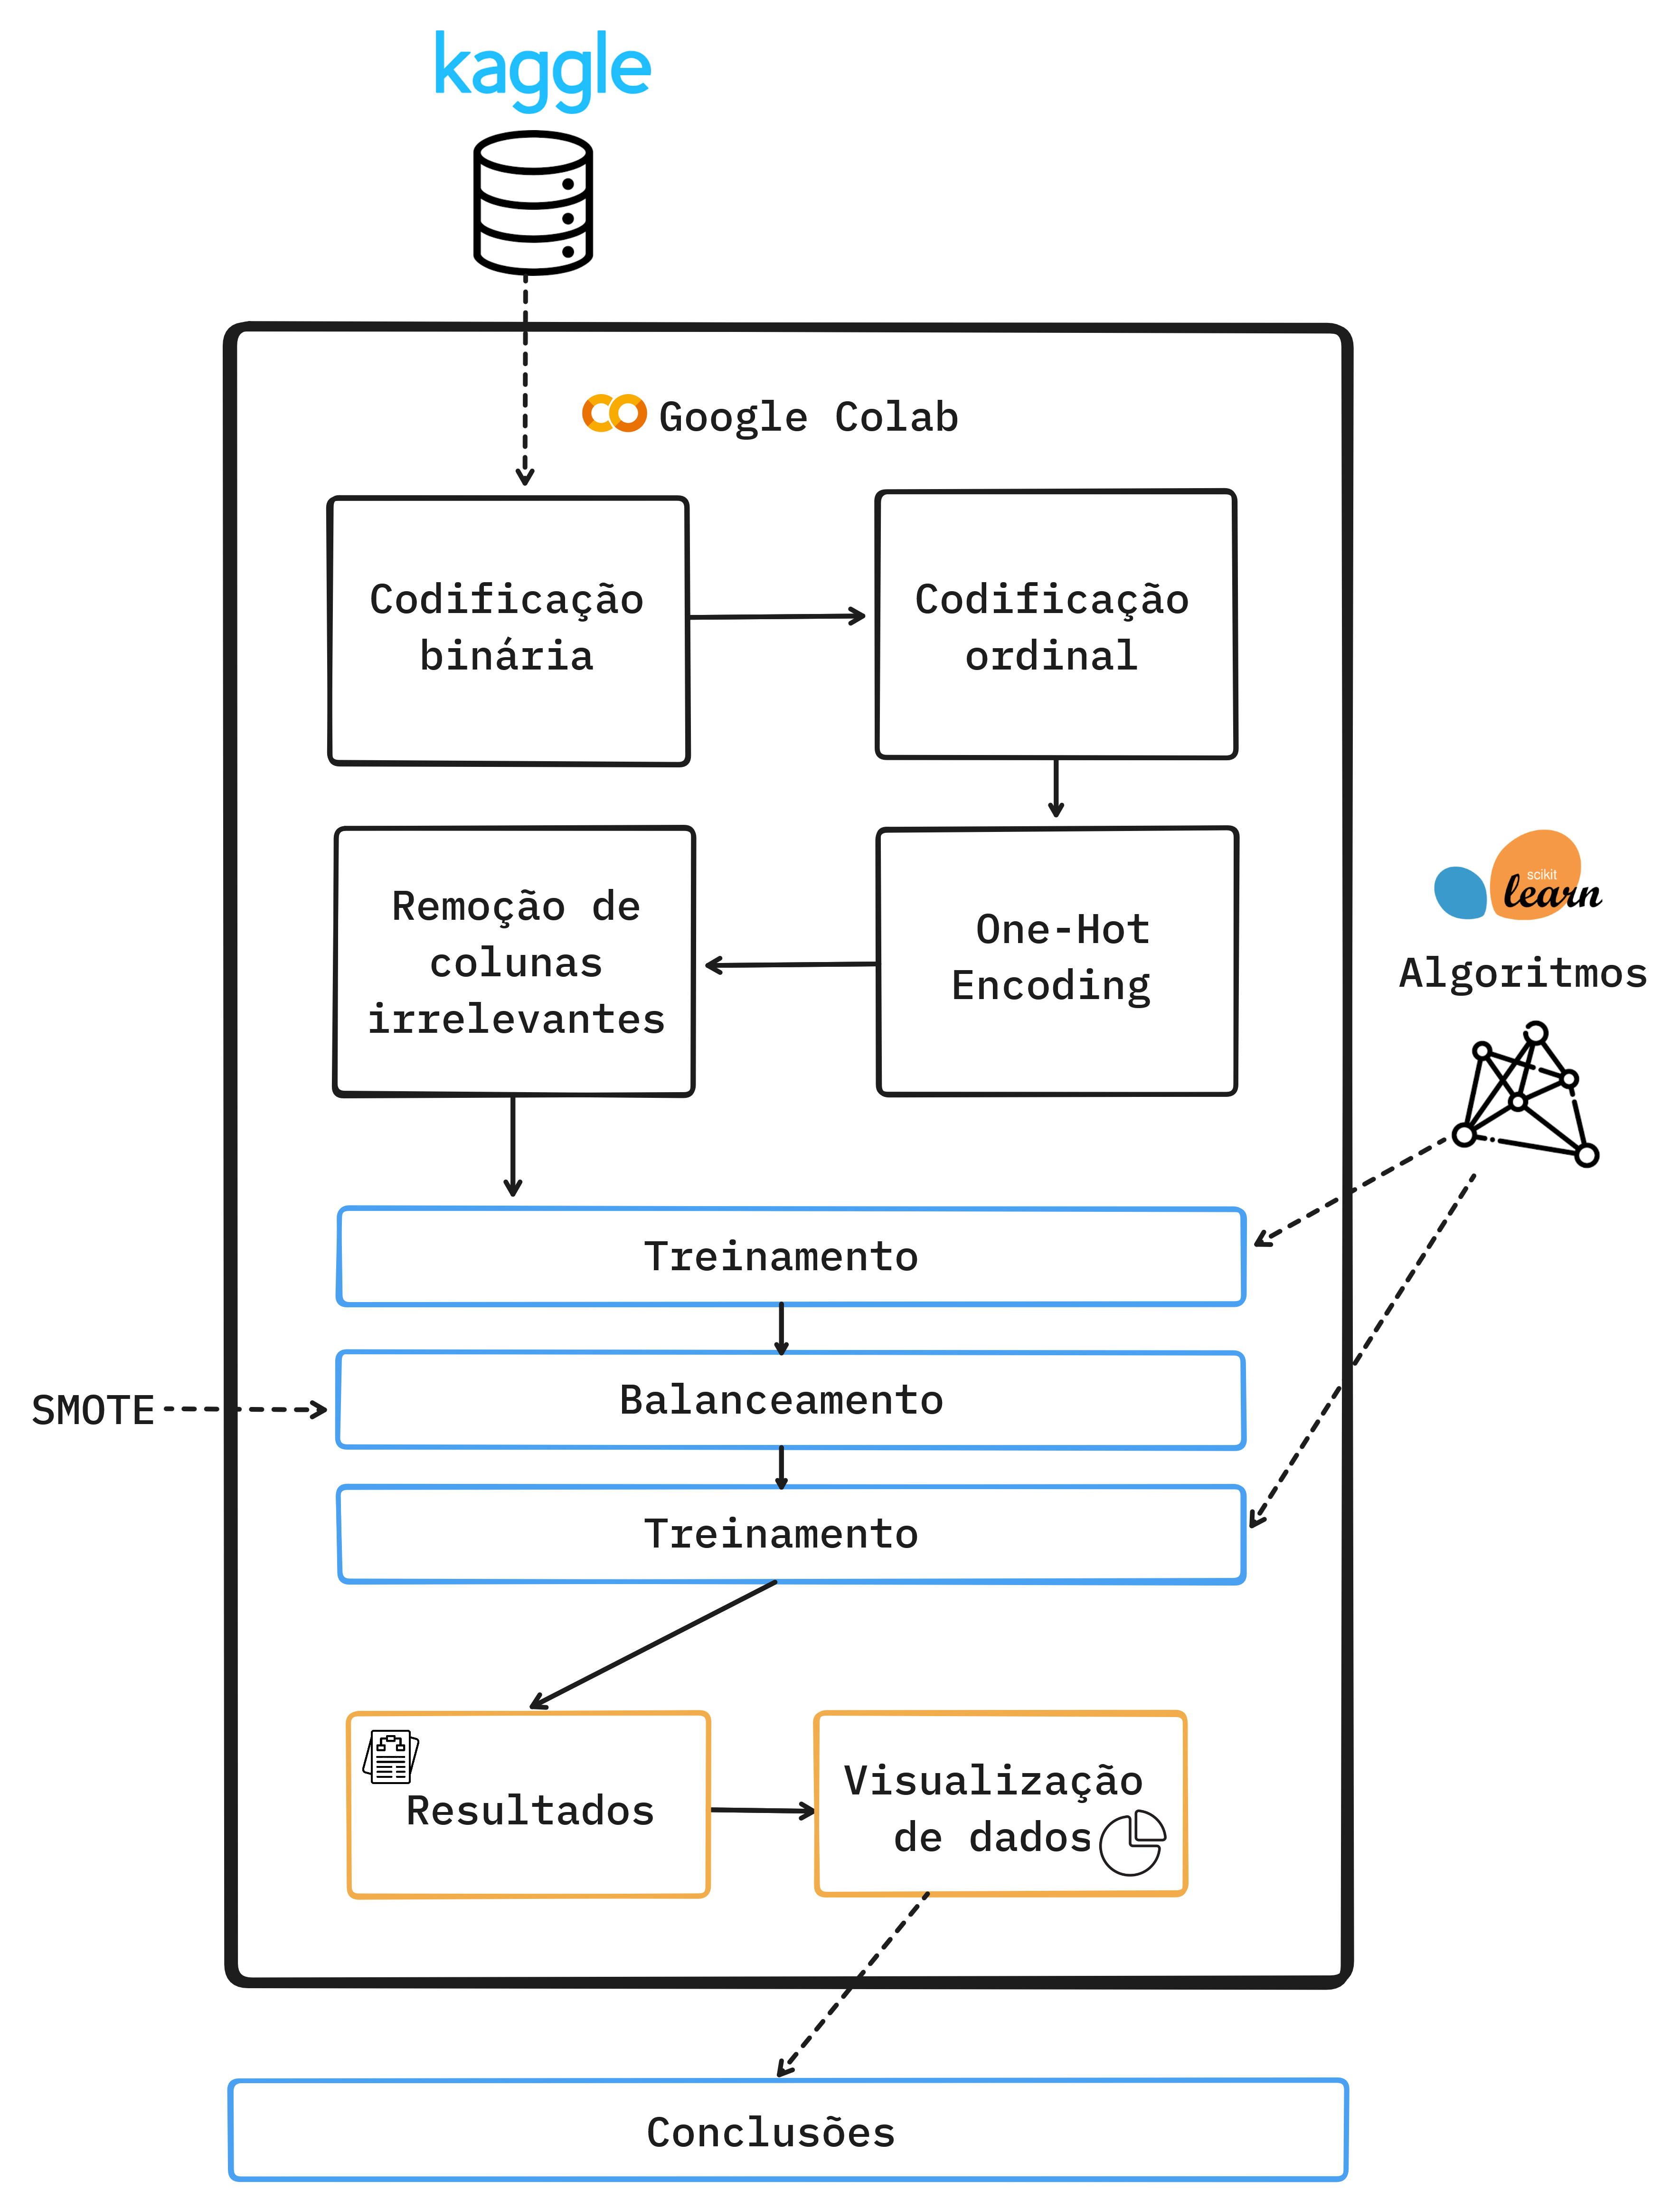
\includegraphics[width=\columnwidth]{methodology.png}
  \caption{Visão geral da metodologia}
  \label{fig:methodology}
\end{figure}

A Figura \ref{fig:methodology} esquematiza as etapas do desenvolvimento metodológico do experimento, que são detalhadas nas seções a seguir.

\subsection{Instrumentos}
Realizou-se a execução do experimento a partir do Google Colab, com apoio de Jupyter Notebooks para documentação. Foram utilizadas as seguintes bibliotecas da linguagem Python: Pandas, para manipulação de dados; Scikit-Learn, para obtenção de modelos e métricas; ImbLearn, para balanceamento de dados.

A seleção dessas ferramentas se deve à sua adequação à manipulação de dados estruturados, bem como à implementação de algoritmos de inteligência artificial no caso do Scikit-Learn, sendo amplamente empregadas em pesquisas na área de aprendizado de máquina.

Como objeto de estudo, escolheu-se o conjunto de dados ``\textit{Vehicle Insurance Claim Fraud Detection}'' \cite{b10}, obtido via Kaggle, que apresenta índice de usabilidade 9.41, garantindo suficiente completude, credibilidade e adequação de formato. A base de dados possui 33 atributos (colunas) e 15.420 instâncias.

\subsection{Métodos}
A importação e manipulação dos dados foram realizadas utilizando a biblioteca Pandas. No pré-processamento, foram aplicadas as seguintes técnicas:
\begin{enumerate}
    \item Codificação binária para variáveis categóricas de dois valores únicos, excluindo a variável-alvo \verb|FraudFound_P|, facilitando a interpretação dos algoritmos, que conseguem lidar melhor com valores binários;
    \item Codificação ordinal para variáveis com ordem natural, transformando-as em valores inteiros e permitindo que os algoritmos aprendam mais facilmente sua progressão;
    \item \textit{One-Hot Encoding} para categorias sem ordenação intrínseca (como \verb|Make|, \verb|MaritalStatus|) a fim de evitar que os algoritmos interpretem erroneamente uma ordem inexistente entre seus valores;
    \item Remoção de colunas irrelevantes para o experimento (\verb|policyNumber|, \verb|Month|, \verb|WeekOfMonth|), que representavam indicadores únicos ou valores redundantes.
\end{enumerate}

Em seguida, os dados foram divididos em conjuntos na proporção de 80\% para treino e 20\% para teste. Essa divisão apresentou resultados relativamente superiores quando comparada a outras proporções testadas em fases preliminares deste estudo. Ressalta-se ainda que a divisão 80/20 é amplamente utilizada na literatura de aprendizado de máquina, proporcionando um bom equilíbrio entre a quantidade de dados para ajuste do modelo e volume suficiente para uma avaliação confiável do desempenho \cite{b8},\cite{b9}. Adicionalmente, visando atingir o terceiro objetivo deste experimento, utilizou-se o algoritmo SMOTE \cite{b5} para balanceamento de dados via superamostragem (do inglês \textit{oversampling}) do conjunto de treino, visando manipular a variável-alvo (\verb|FraudFound_P|) — inicialmente desbalanceada. O SMOTE foi escolhido pois, ao gerar exemplos sintéticos da classe minoritária, permite aumentar a diversidade dos dados e reduzir o risco de sobreajuste (do inglês \textit{overfitting}) associado à replicação simples, sendo apropriado mesmo em conjuntos de dados pequenos e altamente desbalanceados, como demonstrado no estudo de Chawla et al. (2002)\cite{b5}.

A fim de realizar a avaliação dos modelos, atendendo ao primeiro e segundo objetivos específicos deste escopo, foram utilizados quatro algoritmos de aprendizado de máquina supervisionado, obtidos a partir da biblioteca \textit{Scikit-Learn}: Regressão Logística (\verb|LogisticRegression|), \textit{Naïve} Bayes (\verb|GaussianNB|), \textit{\textit{Random Forest} Classifier} (\verb|RandomForestClassifier|), que implementa a Floresta de Decisão, e \textit{Support Vector Classifier} (\verb|SVC RBF Kernel|), que implementa o SVM. No caso do SVC, foi utilizado o \textit{kernel} RBF por ser recomendado na literatura como escolha padrão para problemas gerais de classificação, devido à sua robustez e capacidade de capturar relações não lineares. Outros \textit{kernels}, como o Polinomial e o Sigmoid, são indicados apenas para contextos específicos, pois podem trazer complexidade ou instabilidade ao modelo \cite{b7}.

Cada modelo foi treinado em duas condições distintas: primeiramente, com o conjunto de dados original (desbalanceado) e, depois, com os dados balanceados via SMOTE, permitindo a análise do impacto do balanceamento no desempenho. A Regressão Logística foi configurada para realizar, no máximo, 10000 iterações a fim de garantir convergência, ou seja, assegurar que o algoritmo tenha oportunidades suficientes para ajustar seus parâmetros até encontrar uma solução estável e adequada ao problema. O número elevado de iterações é importante em conjuntos de dados pequenos, nos quais a generalização do modelo pode ser instável e o processo de otimização pode demorar mais para atingir um ponto ótimo. Valores menores de iteração podem resultar em treinamento incompleto, levando a métricas nulas ou insatisfatórias. O SVC e o \textit{Naïve} Bayes utilizaram os parâmetros padrão conforme disponibilizados pela fonte. A separação entre \textit{features} e a variável-alvo foi realizada antes do treinamento, seguindo a divisão prévia em conjuntos de treino e teste (80/20). 

\subsection{Métricas de avaliação}
A avaliação dos modelos baseou-se em quatro métricas: acurácia, precisão, revocação (do inglês \textit{recall}) e F1-score, calculadas por meio da biblioteca \textit{Scikit-Learn}. Tais métricas de avaliação foram escolhidas devido ao sólido embasamento de sua aplicação na literatura, conforme aplicadas Elhusseny et al. (2022)\cite{b6} na metodologia de um estudo semelhante. Essas métricas fornecem diferentes visões de desempenho dos modelos, da seguinte maneira: A \textbf{acurácia} mede a proporção geral de previsões corretas, tanto de fraudes, quanto de não fraudes; a \textbf{precisão} avalia a confiabilidade das predições positivas para fraude (classe minoritária); a \textbf{revocação} mede capacidade de identificar casos de fraude, ainda que sejam falsos-positivos; e, por fim, o \textbf{F1-score} combina as métricas de precisão e revocação em um único indicador, sendo útil para comparar modelos em problemas onde uma classe minoritária é de interesse primário, como o apresentado neste estudo, promovendo equilíbrio entre detectar fraudes de forma geral e minimizar o alerta para transações legítimas.

\section{Resultados}

Os resultados obtidos a partir da aplicação dos modelos de aprendizado de máquina são apresentados a seguir, considerando as quatro métricas de desempenho avaliadas. Conforme sumarizados os valores na Tabela \ref{tab:resultados_desbalanceados}, a princípio, conduziu-se a análise sobre conjunto de dados original, sem aplicação de balanceamento. As Figuras \ref{fig:accuracy_no_smote}, \ref{fig:precision_no_smote}, \ref{fig:recall_no_smote} e \ref{fig:f1_no_smote} ilustram o desempenho de acurácia, precisão, revocação e F1-score, respectivamente.

\begin{table}[h]
\centering
\caption{Desempenho dos modelos no conjunto de dados desbalanceado}
\label{tab:resultados_desbalanceados}
    \begin{tabular}{lcccc}
        \hline
        Modelo & Acurácia & Precisão & Revocação & F1-Score \\ \hline
        Regressão Logística & 0.9403 & 0.3750 & 0.0165 & 0.0316 \\
        \textit{Naïve} Bayes & 0.1560 & 0.0641 & 0.9780 & 0.1203 \\
        SVM (RBF Kernel) & 0.9407 & 0.4800 & 0.0659 & 0.1159 \\
        \textit{Random Forest Classifier}& 0.9426 & 0.7778 & 0.0385 & 0.0733 \\
    \end{tabular}
\end{table}

\begin{figure}[h]
    \centering
    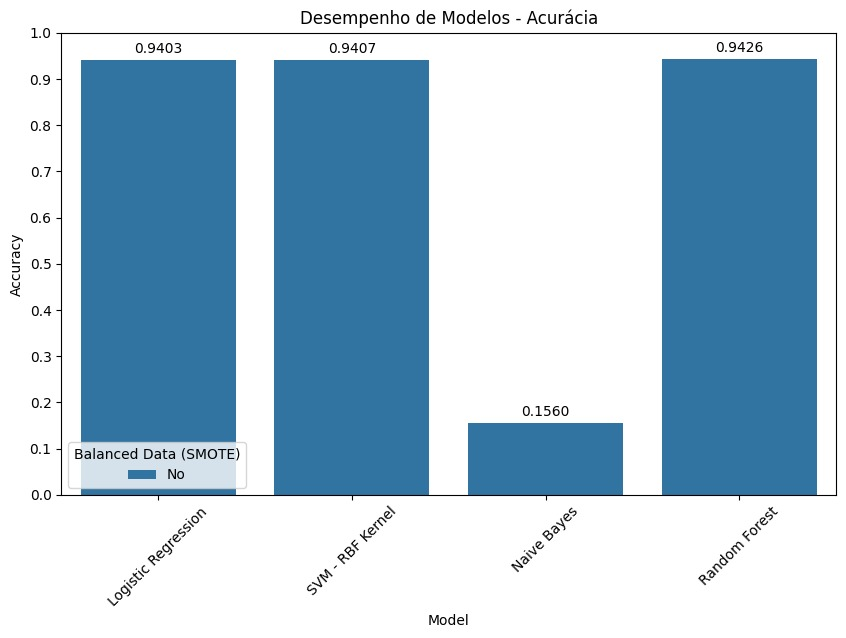
\includegraphics[width=0.9\linewidth]{no_smote_accuracy.jpg}
    \caption{Desempenho da métrica de Acurácia nos dados desbalanceados.}
    \label{fig:accuracy_no_smote}
\end{figure}

\begin{figure}[h]
    \centering
    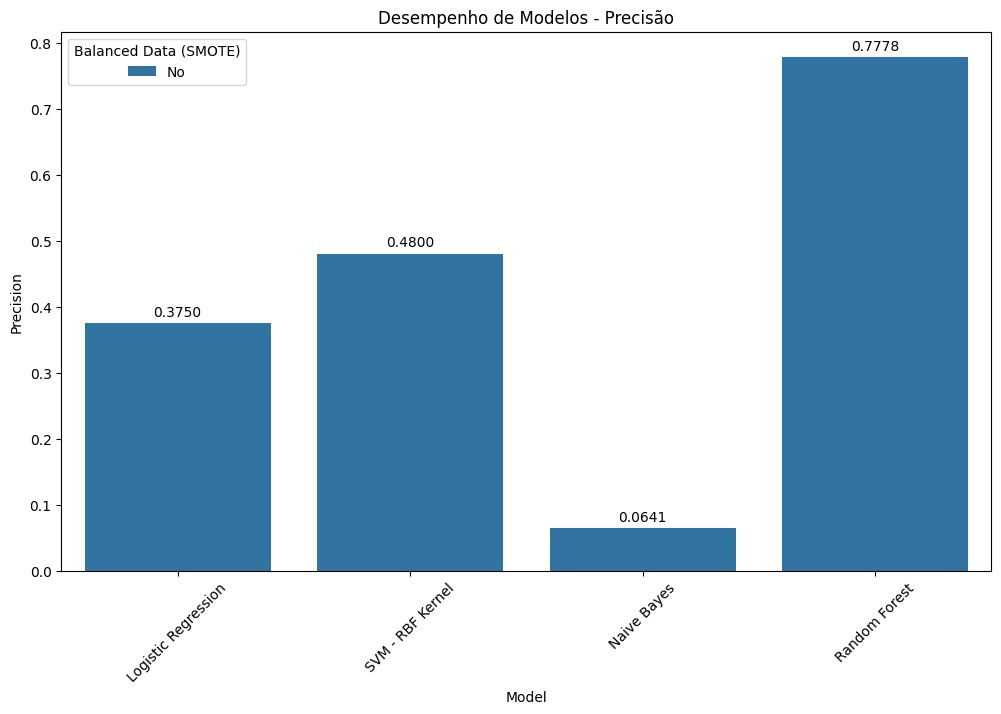
\includegraphics[width=0.9\linewidth]{no_smote_precision.jpg}
    \caption{Desempenho da métrica de Precisão nos dados desbalanceados.}
    \label{fig:precision_no_smote}
\end{figure}

\begin{figure}[h]
    \centering
    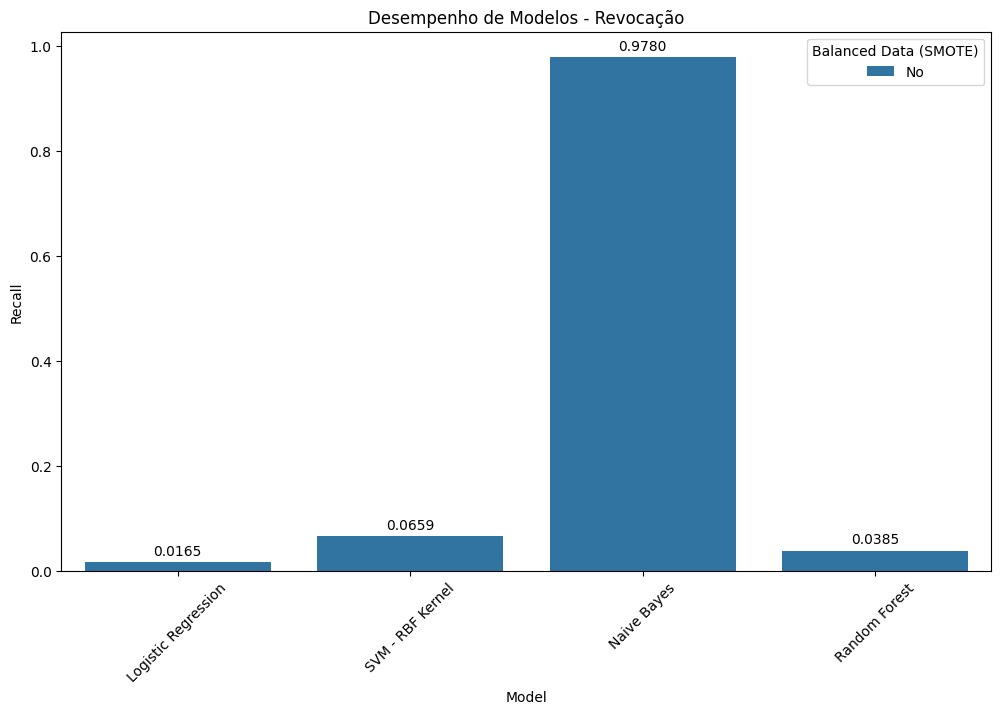
\includegraphics[width=0.9\linewidth]{no_smote_recall.jpg}
    \caption{Desempenho da métrica de Revocação nos dados desbalanceados.}
    \label{fig:recall_no_smote}
\end{figure}

\begin{figure}[ht]
    \centering
    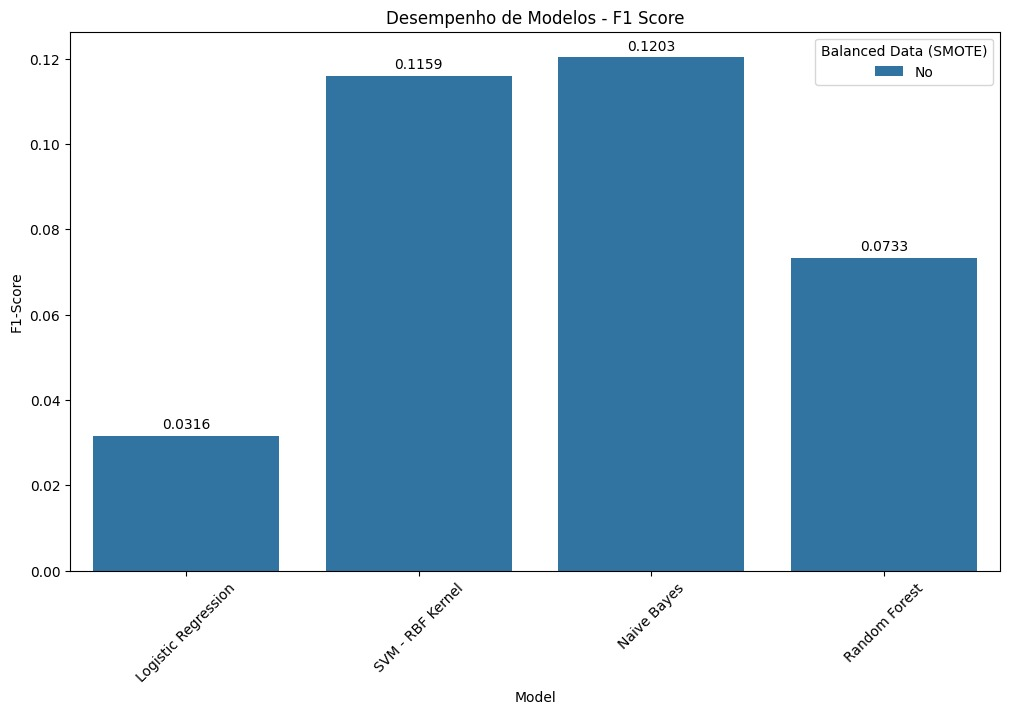
\includegraphics[width=0.9\linewidth]{no_smote_f1.jpg}
    \caption{Desempenho da métrica de F1-Score nos dados desbalanceados.}
    \label{fig:f1_no_smote}
\end{figure}


Em relação à acurácia, observa-se que os modelos \textit{Random Forest Classifier} (0,9426), SVM (0,9407) e Regressão Logística (0,9403) apresentaram desempenhos muito similares. O modelo \textit{Naïve} Bayes, contudo, apresentou acurácia significativamente inferior (0,1560), indicando capacidade reduzida para capturar corretamente os padrões presentes nos dados. 

Em termos de precisão, o modelo \textit{Naïve} Bayes apresentou desempenho inferior aos demais (0,0641), indicando uma alta taxa de falsos positivos. Embora tenha alcançado uma revocação muito elevada (0,9780), detectando quase todos os casos de fraude, o excesso de falsos positivos compromete sua praticidade em cenários reais. Consequentemente, o alto \textit{score} de revocação do \textit{Naïve} Bayes levou a um F1-Score (0,1203) também superior à performance dos demais modelos. 

De modo geral, o  \textit{Random Forest Classifier} (0,0733) se destacou como o modelo mais equilibrado, com desempenho consistentemente superior em três das quatro métricas avaliadas. Com exceção do \textit{Naïve} Bayes, é possível observar que os modelos priorizam o julgamento correto da classe majoritária (transações legítimas) em detrimento de uma detecção mais abrangente que levasse a mais falsos positivos.

Posteriormente, realizou-se o treinamento dos modelos, sob os mesmos parâmetros, com o conjunto de dados balanceado via SMOTE. Os resultados obtidos estão sumarizados na Tabela \ref{tab:resultados_balanceados}. As Figuras \ref{fig:accuracy_smote}, \ref{fig:precision_smote}, \ref{fig:recall_smote} e \ref{fig:f1_smote} apresentam, respectivamente, os desempenhos de acurácia, precisão, revocação e F1-score com a aplicação do SMOTE.

\begin{table}[h]
    \centering
    \caption{Desempenho dos modelos no conjunto de dados balanceado}
    \label{tab:resultados_balanceados}
    \begin{tabular}{lcccc}
    \hline
    Modelo & Acurácia & Precisão & Revocação & F1-Score \\ \hline
    Regressão Logística & 0.9403 & 0.3750 & 0.0165 & 0.0316 \\
    \textit{Naïve} Bayes & 0.2007 & 0.0655 & 0.9451 & 0.1225 \\
    SVM (RBF Kernel) & 0.9400 & 0.4444 & 0.0659 & 0.1148 \\
    \textit{Random Forest Classifier}& 0.9410 & 0.5000 & 0.0495 & 0.0900 \\
    \end{tabular}
\end{table}

\begin{figure}[h]
    \centering
    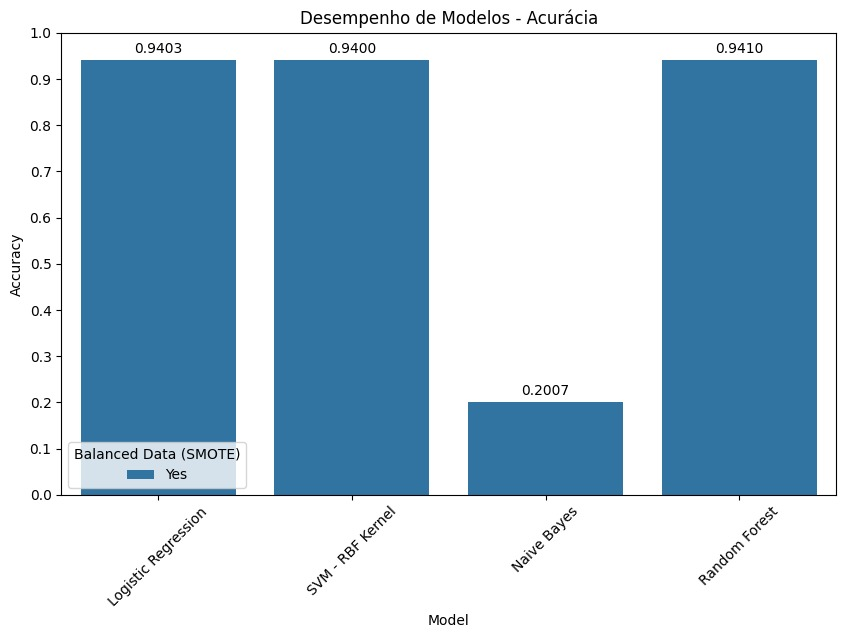
\includegraphics[width=0.9\linewidth]{smote_accuracy.jpg}\textbf{}
    \caption{Desempenho da métrica de Acurácia nos dados balanceados com SMOTE.}
    \label{fig:accuracy_smote}
\end{figure}

\begin{figure}[h]
    \centering
    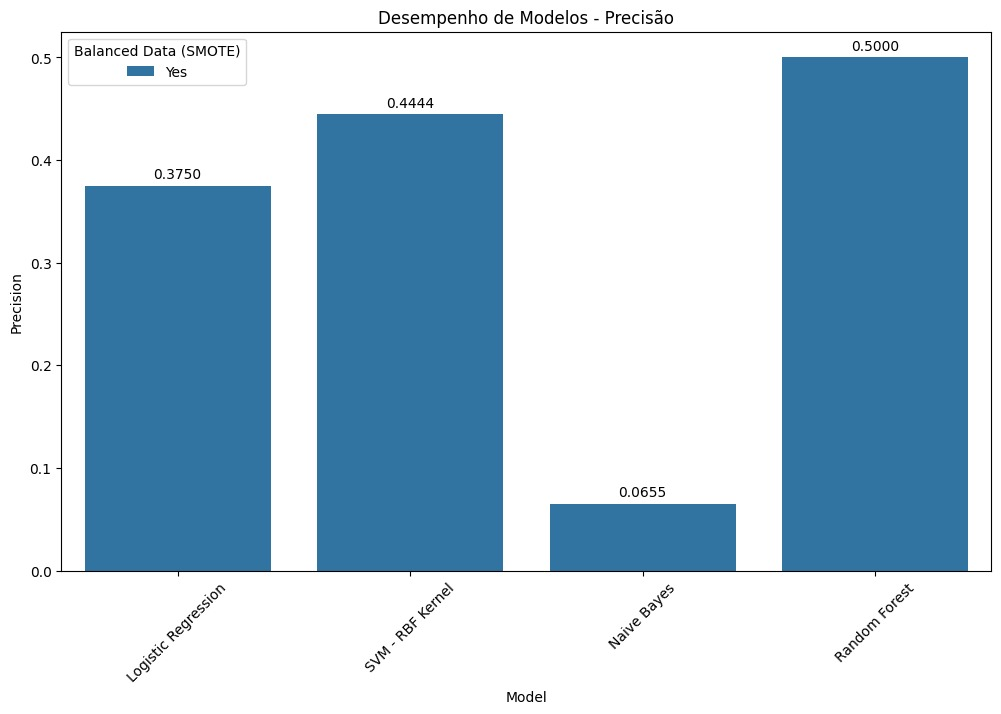
\includegraphics[width=0.9\linewidth]{smote_precision.jpg}
    \caption{Desempenho da métrica de Precisão nos dados balanceados com SMOTE.}
    \label{fig:precision_smote}
\end{figure}

\begin{figure}[h]
    \centering
    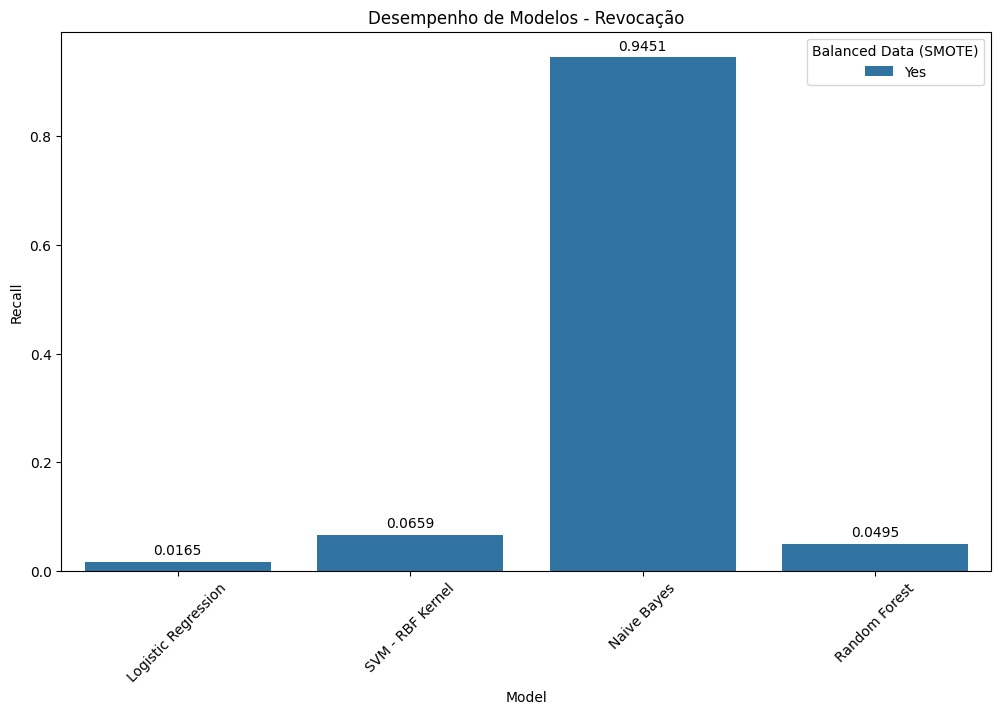
\includegraphics[width=0.9\linewidth]{smote_recall.jpg}
    \caption{Desempenho da métrica de Revocação nos dados balanceados com SMOTE.}
    \label{fig:recall_smote}
\end{figure}

\begin{figure}[ht]
    \centering
    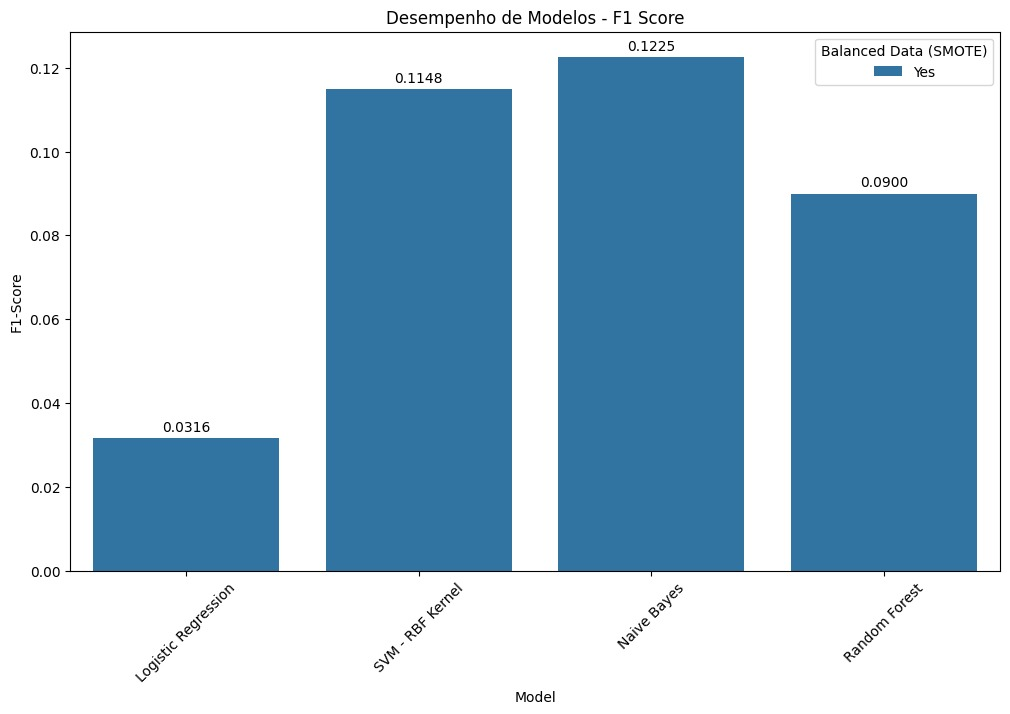
\includegraphics[width=0.9\linewidth]{smote_f1.jpg}
    \caption{Desempenho da métrica de F1-Score nos dados balanceados com SMOTE.}
    \label{fig:f1_smote}
\end{figure}

Em relação à acurácia, observa-se que os modelos de Regressão Logística (0,9403), SVM (0,9400) e \textit{Random Forest} (0,9410) mantiveram desempenho semelhante, mesmo após o balanceamento dos dados. Isso sugere que o balanceamento não impactou significativamente a capacidade desses modelos de classificar corretamente cerca de 94\% das instâncias.

Por outro lado, o modelo \textit{Naïve} Bayes apresentou acurácia notoriamente baixa (0,2007), indicando que o modelo permaneceu com dificuldades para capturar os padrões gerais dos dados, ainda que agora balanceados. No que se refere à precisão, o \textit{Naïve} Bayes manteve desempenho inferior (0,0655) em comparação aos outros modelos, evidenciando a persistência de um número elevado de falsos positivos.  

Analisando a revocação, o \textit{Naïve} Bayes novamente apresentou desempenho significativamente superior aos demais (0,9451). No entanto, considerando sua precisão baixa, a aplicabilidade prática desse modelo é limitada. Os demais modelos apresentaram revocações baixas, com valores entre 0,0165 (Regressão Logística) e 0,0659 (SVM), o que leva à conclusão de que continuam priorizando a classe majoritária, mesmo após o balanceamento. 

Por fim, visando alcançar o terceiro objetivo específico dessa pesquisa, foi realizada uma comparação da variação de cada métrica após o balanceamento de dados, conforme se verifica na Tabela \ref{tab:variacao_balanceamento}.

\begin{table}[h]
\centering
\caption{Variação percentual após balanceamento dos dados}
\label{tab:variacao_balanceamento}
    \begin{tabular}{lcc}
    \hline
    \textbf{Modelo} & \textbf{Acurácia (\%)} & \textbf{Precisão (\%)} \\ \hline
    Regressão Logística & 0.00 & 0.00 \\
    \textit{Naïve} Bayes         & +28.69 & +2.18 \\
    SVM (RBF Kernel)    & -0.07  & -7.42 \\
    \textit{Random Forest Classifier}& -0.17  & -35.71 \\ \hline
    \textbf{Média}      & \textbf{+9.48} & \textbf{-13.65} \\ \hline
    \end{tabular}
    
    \vspace{0.3cm}
    
    \begin{tabular}{lcc}
    \hline
    \textbf{Modelo} & \textbf{Revocação (\%)} & \textbf{F1-Score (\%)} \\ \hline
    Regressão Logística & 0.00 & 0.00 \\
    \textit{Naïve} Bayes         & -3.36 & +1.83 \\
    SVM (RBF Kernel)    & 0.00  & -0.95 \\
    \textit{Random Forest Classifier}& +28.57 & +22.78 \\ \hline
    \textbf{Média}      & \textbf{+8.40} & \textbf{+7.88} \\ \hline
    \end{tabular}
\end{table}

A análise das variações evidencia que o balanceamento dos dados gerou impactos significativos em alguns modelos, ainda que de modo inconsistente entre as métricas. O \textit{Naïve} Bayes apresentou a maior variação positiva em acurácia (+28,69\%), embora permanecendo com desempenho geral insatisfatório. 

Em contraste, o \textit{Random Forest Classifier} obteve uma queda acentuada na precisão (-35,71\%), indicando aumento expressivo de falsos positivos após o balanceamento. Contudo, foi o que mais se beneficiou em termos de revocação (+28,57\%) e F1-score (+22,78\%), sugerindo que o SMOTE ampliou sua capacidade de identificar fraudes sem sacrificar completamente o equilíbrio entre classes. 

Esses resultados destacam que, embora o balanceamento possa melhorar aspectos específicos do desempenho, seus efeitos são altamente dependentes do modelo e da métrica considerada.

\section{Conclusões}

De forma geral, os modelos Regressão Logística, SVM e \textit{Random Forest Classifier} apresentaram acurácias elevadas e relativamente consistentes antes e após o balanceamento, com valores próximos de 94\%. O modelo \textit{Random Forest Classifier}, apesar de não atingir revocações elevadas, manteve-se como o mais equilibrado em termos gerais, indicando ser uma opção adequada para cenários em que se busca um compromisso mais balanceado entre detecção de fraude e controle de falsos positivos. No que se refere à revocação, o modelo \textit{Naïve} Bayes se destacou, atingindo 97,80\% no conjunto desbalanceado e 94,51\% no balanceado, indicando uma alta capacidade de identificar casos de fraude de forma geral. Contudo, esse desempenho foi acompanhado de uma precisão baixa em relação aos demais, o que leva a inferência de um elevado número de falsos positivos. Tal comportamento reflete-se também em seu F1-score, que, apesar superior ao dos demais modelos, reforça a existência de um forte \textit{trade-off} entre revocação e precisão. 

Na prática, no contexto da indústria de seguros automotivos, a utilização do modelo \textit{Naïve} Bayes se comprova menos recomendada em relação aos demais devido a seu número excessivo de falsos positivos, implicando potenciais custos operacionais elevados, visto que suspeitas de fraudes geram a necessidade de investigações e recursos que podem ser equivocadamente destinados a transações legítimas classificadas como fraudulentas. Nesse sentido, embora uma alta revocação seja desejável em de detecção de fraude, ela não pode ser analisada de forma isolada, especialmente quando acompanhada de uma disparidade de precisão, como a observada no \textit{Naïve} Bayes neste experimento.

Portanto, conclui-se que, de modo geral, para a tarefa de detecção de fraudes em seguros automotivos, modelos baseados em \textit{Random Forest} ou SVM oferecem maior eficácia quando comparados ao \textit{Naïve} Bayes, especialmente sob a perspectiva dos possíveis custos associados à gestão de muitos falsos positivos. Já o modelo de Regressão Logística, apesar de demonstrar alta acurácia, obteve desempenho consideravelmente inferior aos demais no que se refere à F1-Score, sendo assim menos indicado para esse contexto.

Como trabalhos futuros, sugere-se a exploração outras técnicas aplicadas para detecção de fraudes automotivas, como redes neurais profundas, bem como a reprodução deste experimento sob outros métodos para tratamento de desbalanceamento.

\section*{Referências}

\begin{thebibliography}{00}
\bibitem{b1} McKinsey \& Company, Global Insurance Report 2025: The pursuit of growth. 2024. Disponível em: \url{https://www.mckinsey.com/industries/financial-services/our-insights/global-insurance-report}. Acesso em 13 de maio de 2025.
\bibitem{b2} PressWorks,  ``Tendências no mercado de Seguros Auto em 2025'', \textit{Valor Econômico}, Jan. 20, 2025. Disponível em: \url{https://valor.globo.com/patrocinado/pressworks/noticia/2025/01/20/tendencias-no-mercado-de-seguros-auto-em-2025.ghtml}. Acesso em 13 de maio de 2025.
\bibitem{b3} D. Multas,  ``Quais são as fraudes mais comuns em seguros ou proteções veiculares e como evitar?'', \textit{JusBrasil}, Nov. 6, 2019. Disponível em: \url{https://www.jusbrasil.com.br/artigos/quais-sao-as-fraudes-mais-comuns-em-seguros-ou-protecoes-veiculares-e-como-evitar/777802680}. Acesso em 25 de maio de 2025.
\bibitem{b4} F. K. Alarfaj, I. Malik, H. U. Khan, N. Almusallam, M. Ramzan, and M. Ahmed, ``Credit card fraud detection using state-of-the-art machine learning and deep learning algorithms'', IEEE Access, vol. 10, pp. 39700–39715, 2022, doi: 10.1109/ACCESS.2022.3166891.
\bibitem{b5} N. V. Chawla, K. W. Bowyer, L. O. Hall, and W. P. Kegelmeyer, ``SMOTE: Synthetic Minority Over-sampling Technique'', \textit{Journal of Artificial Intelligence Research}, vol. 16, pp. 321–357, 2002. doi: 10.1613/jair.953. 
\bibitem{b6} N. S. Elhusseny, S. M. Ouf, and A. M. Idrees, ``Credit Card Fraud Detection Using Machine Learning Techniques'', \textit{Future Computing and Informatics Journal}, vol. 7, no. 1, Article 2, 2022. doi: 10.54623/fue.fcij.7.1.2. 
\bibitem{b7}
C.-W. Hsu, C.-C. Chang, and C.-J. Lin, ``\textit{{A Practical Guide to Support Vector Classification}}'', Department of Computer Science, National Taiwan University, 2016. 
\bibitem{b8}
A. Géron, \textit{Hands-On Machine Learning with Scikit-Learn, Keras, and TensorFlow}, 2nd ed., O’Reilly Media, 2019.
\bibitem{b9}
G. James, D. Witten, T. Hastie, and R. Tibshirani, \textit{An Introduction to Statistical Learning: with Applications in R}, Springer, 2013.
\bibitem{b10} 
S. Bansal, “Vehicle Insurance Claim Fraud Detection,” \textit{Kaggle}, [Online]. Available: \url{https://www.kaggle.com/datasets/shivamb/vehicle-claim-fraud-detection}.
\end{thebibliography}
\vspace{12pt}

\end{document}
